\documentclass[10pt]{beamer}

\usepackage{presentation}

\usetheme{Madrid}
\setbeamersize{text margin left=30pt,text margin right=20pt}
\graphicspath{{../figures/}}

\usepackage[backend=biber,style=authoryear-comp]{biblatex}
\addbibresource{references.bib}

% Beamer needs this to show footnotes properly.
\setbeamertemplate{footnote}{%
  \parindent 0em\noindent
  \raggedright
  \insertfootnotemark\insertfootnotetext\par
}
\setbeamertemplate{bibliography item}[triangle]
\setbeamertemplate{itemize item}[triangle]
\setbeamertemplate{itemize subitem}[circle]
\setbeamerfont{bibliography item}{size=\scriptsize}
\setbeamerfont{bibliography entry author}{size=\scriptsize}
\setbeamerfont{bibliography entry title}{size=\scriptsize}
\setbeamerfont{bibliography entry location}{size=\scriptsize}
\setbeamerfont{bibliography entry note}{size=\scriptsize}

% Colors retained from the supplied template.
\definecolor{codegreen}{RGB}{34,139,34}
\definecolor{codegray}{RGB}{120,120,120}
\definecolor{codeblue}{RGB}{0,92,175}
\definecolor{codepurple}{RGB}{163,21,21}
\definecolor{backcolour}{RGB}{248,248,248}
\definecolor{accent}{RGB}{42,63,95}
\definecolor{muted}{RGB}{105,105,105}
\definecolor{rulegray}{RGB}{205,210,218}

% Title page
\title[Trajectory Prediction]{Inferring Launch and Environmental Parameters from Simulated Trajectories}
\subtitle{Machine Learning for Quantum Scientists (physics7516)}
\author{Leon Galbas}
\date{31/07/2026}
\institute[Universität Bonn]{Rheinische Friedrich-Wilhelms-Universität Bonn}

\begin{document}

\begin{frame}[plain]
  \titlepage
\end{frame}

% Table of Contents
\begin{frame}{Outline}
    \tableofcontents
\end{frame}
% Current section
\AtBeginSection[ ]
{
\begin{frame}{Outline}
    \tableofcontents[currentsection]
\end{frame}
}

\section{Problem idea and data generation}

\begin{frame}{Can launch parameters be inferred from object trajectories?}
  \vspace{0.35cm}
  \[
    \text{trajectory } \bigl\{\vb{r}(t_1),\ldots,\vb{r}(t_T)\bigr\}
    \;\longrightarrow \;
    \text{ML model}
    \; \longrightarrow \;
    \text{launch parameters } \widehat{\vb{\lambda}}
  \]

  \vspace{0.45cm}
  \[
    \vb{\lambda} = \big(
      \underbrace{v_x,v_y,v_z,}_{\shortstack{initial\\velocity}}\;
      \underbrace{u_x,u_y,u_z,}_{\shortstack{wind\\velocity}}\;
      \underbrace{\omega_x,\omega_y,\omega_z,}_{\shortstack{rotation\\axis}}\;
      \underbrace{\beta_D,\beta_M}_{\shortstack{drag and\\Magnus\\parameters}}
    \big)
  \]
\end{frame}

\begin{frame}{Simulated trajectories}
    \begin{figure}[h]
        \centering
        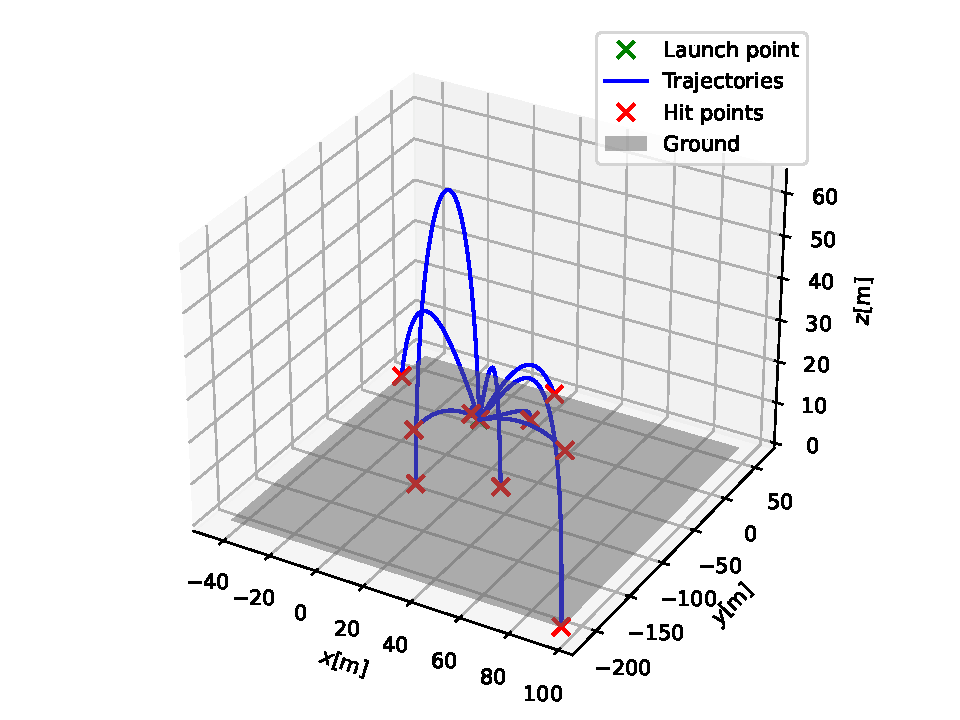
\includegraphics[width=\linewidth,height=0.70\textheight,keepaspectratio]{sample_trajectories_3d.pdf}
        \caption{Ten exemplary simulated trajectories.}
    \end{figure}
\end{frame}

\begin{frame}{Equations of motion}
  \vspace{0.25cm}
  \[
    \dv{\vb{r}}{t}=\vb{v},
    \qquad
    \dv{\vb{v}}{t}
    =
    \underbrace{\vb{g}}_{\text{gravity}}
    -
    \underbrace{\beta_D\abs{\vb{q}}\vb{q}}_{\text{drag}}
    +
    \underbrace{\beta_M
      \l(\widehat{\vb{\omega}}\times\vb{q}\r)}_{\text{Magnus}},
    \qquad
    \vb{q}=\vb{v}-\vb{u}.
  \]

  \vspace{0.65cm}
  \begin{itemize}
    \setlength{\itemsep}{0.6em}
    \item $\vb{q}$: velocity relative to the wind
    \item drag: deceleration opposite the relative motion
    \item Magnus term: spin-induced curvature
  \end{itemize}
\end{frame}

\begin{frame}{Simulation parameters}
  \begin{table}
    \centering
    \begin{tabular}{@{}lll@{}}
      \toprule
      Quantity & Symbol & Sampled range \\
      \midrule
      Initial speed & $v_0$ & $\qtyrange{0}{75}{\meter\per\second}$ \\
      Wind speed & $u$ & $\qtyrange{0}{25}{\meter\per\second}$ \\
      Drag strength & $\beta_D$ & $\qtyrange{0.003}{0.04}{\per\meter}$ \\
      Magnus strength & $\beta_M$ & $\qtyrange{0}{0.3}{\per\second}$ \\
      \bottomrule
    \end{tabular}
  \end{table}

  \vspace{0.55cm}
  \[
    \num{200000}\ \text{trajectories}
  \]
  \[
    \num{10000}\ \text{raw points}
    \longrightarrow
    \num{100}\ \text{time points}
  \]

  \begin{center}
    Integrate from launch until the projectile reaches $z=0$.
  \end{center}
\end{frame}

\section{Models}

\begin{frame}{Two model approaches}
  \begin{table}
    \centering
    \begin{tabular}{@{}lll@{}}
      \toprule
      & Engineered features + MLP & Time series + GRU \\
      \midrule
      Input
        & 24 trajectory summaries
        & 100 ordered observations \\
      Examples
        & time, range, apex, derivatives
        & $t,x,y,z$, optionally $\vb{v},\vb{a}$ \\
      Strength
        & compact and interpretable
        & retains temporal structure \\
      \bottomrule
    \end{tabular}
  \end{table}

  \vspace{0.55cm}
  \[
    160{,}000\ \text{training}
    \qquad+\qquad
    40{,}000\ \text{test}
  \]
\end{frame}

\section{Results}

\subsection{On full trajectories}

\begin{frame}{Model performance on full trajectories}
  \begin{table}
    \centering
    \begin{tabular}{@{}lccc@{}}
      \toprule
      Target RMSE & MLP & GRU, position & GRU, derivatives \\
      \midrule
      $v_x\,[\unit{m\,s^{-1}}]$
        & \textcolor{accent}{1.016} & 1.793 & 1.027 \\
      $u_x\,[\unit{m\,s^{-1}}]$
        & 3.857 & 2.667 & \textcolor{accent}{1.359} \\
      $\omega_x$
        & 0.413 & 0.247 & \textcolor{accent}{0.129} \\
      $\beta_D\,[\unit{m^{-1}}]$
        & 0.00445 & 0.00300 & \textcolor{accent}{0.00127} \\
      $\beta_M\,[\unit{s^{-1}}]$
        & 0.0664 & 0.0378 & \textcolor{accent}{0.0190} \\
      \bottomrule
    \end{tabular}
    \caption{Comparison of the prediction performance for selected test set parameters and model configurations.}
  \end{table}
\end{frame}

\subsection{On partial trajectories}

\begin{frame}{Model performance on partial trajectories}
  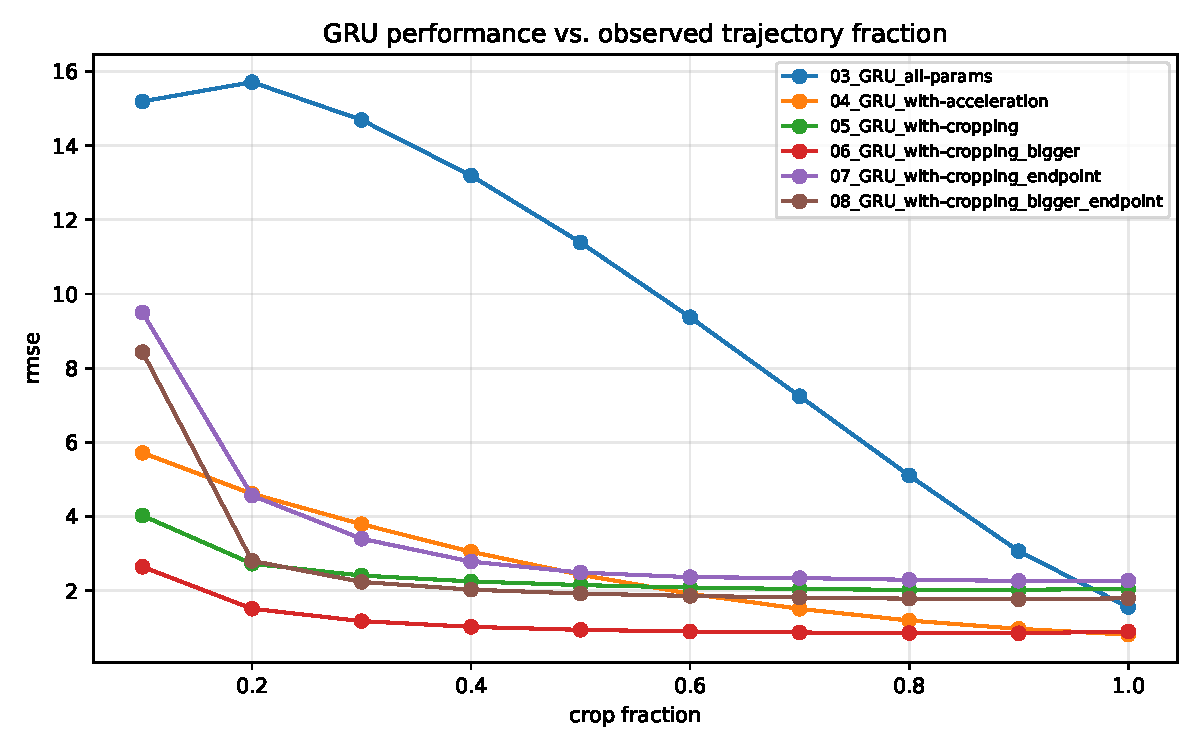
\includegraphics[width=\linewidth,height=0.70\textheight,keepaspectratio]
    {gru_performance_vs_cropping.pdf}
\end{frame}

\begin{frame}{Model performance on partial trajectories}
  \begin{table}
    \centering
    \begin{tabular}{@{}lll@{}}
      \toprule
      Observed fraction & Target & RMSE \\
      \midrule
      $10\%$ & $v_x$, full-flight training
        & $6.62\unit{m\,s^{-1}}$ \\
      $10\%$ & $v_x$, crop training
        & \textcolor{accent}{$2.16\unit{m\,s^{-1}}$} \\
      $50\%$ & $u_x$, crop training
        & $1.64\unit{m\,s^{-1}}$ \\
      $50\%$ & $\beta_M$, crop training
        & $0.0223\unit{s^{-1}}$ \\
      \bottomrule
    \end{tabular}
    \caption{RMSE for selected parameters for Model 04 (derivative-augmented GRU trained on
      complete trajectories) and Model 06 (larger derivative-augmented GRU
      trained with random cropping).}
  \end{table}

  \vspace{0.7cm}
  \begin{center}
    At $10\%$ observation, crop training reduces the
    $v_x$ error by about two thirds.

    The largest cropping gain occurs early in the flight
  \end{center}
\end{frame}

\subsection{On noisy trajectories}

\begin{frame}{Model performance on noisy trajectories}
  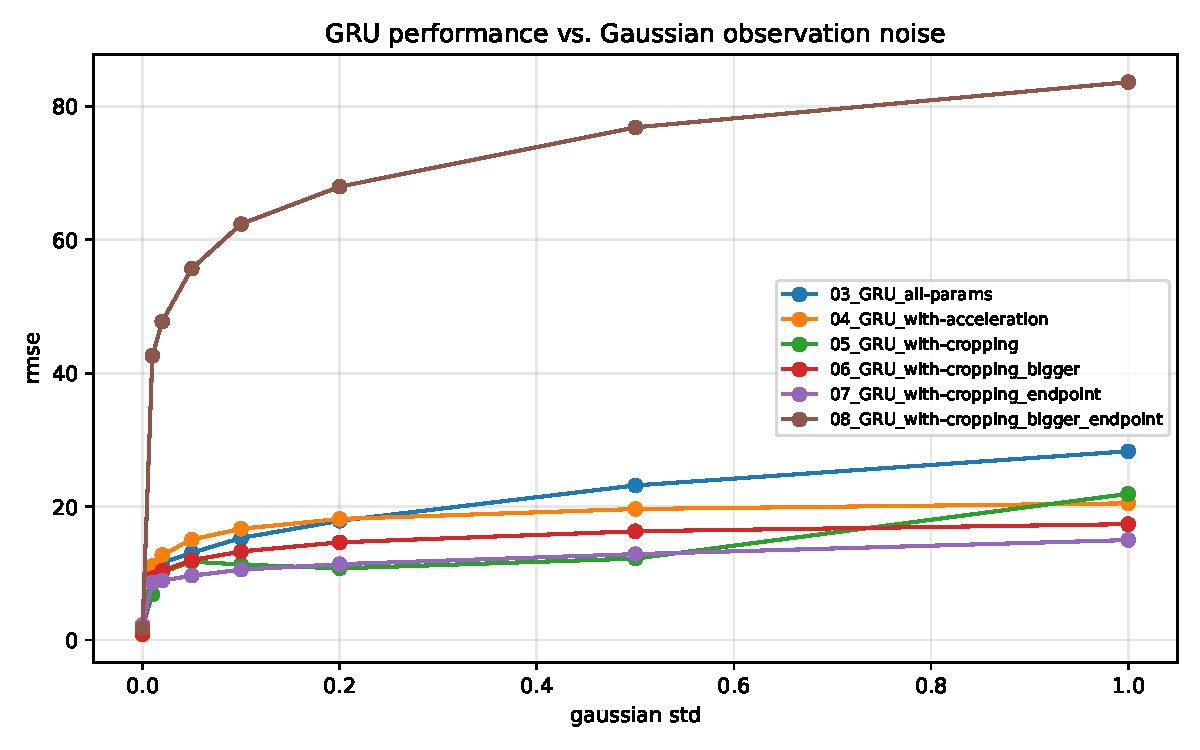
\includegraphics[width=\linewidth,height=0.70\textheight,keepaspectratio]
    {gru_performance_vs_gaussian_noise.pdf}
\end{frame}

\begin{frame}{Model performance on noisy trajectoriese}
  \begin{table}
    \centering
    \begin{tabular}{@{}lccc@{}}
      \toprule
      Target RMSE & Clean & $\sigma=0.01\unit{m}$ & Increase \\
      \midrule
      $v_x\,[\unit{m\,s^{-1}}]$
        & 1.03 & 21.0 & \textcolor{accent}{$20.4\times$} \\
      $u_x\,[\unit{m\,s^{-1}}]$
        & 1.36 & 9.50 & \textcolor{accent}{$7.0\times$} \\
      $\beta_D\,[\unit{m^{-1}}]$
        & 0.00127 & 0.0120 & \textcolor{accent}{$9.4\times$} \\
      \bottomrule
    \end{tabular}
    \caption{Noise robustness of Model 04, the derivative-augmented GRU,
      evaluated on clean positions and with
      \(\sigma=0.01\unit{m}\) positional noise.}
  \end{table}

  \vspace{0.75cm}
  \[
    \text{noisy positions}
    \quad\longrightarrow\quad
    \text{numerical derivatives}
    \quad\longrightarrow\quad
    \text{amplified noise}
  \]
\end{frame}

\section{Conclusion}

\begin{frame}{Conclusion}
  \begin{itemize}
    \setlength{\itemsep}{0.65em}
    \item Engineered features are strongest when they directly encode the target.
    \item GRU derivative inputs best recover the full physics from clean data.
    \item Random-prefix training enables prediction from incomplete flights.
    \item Real measurements require noise-aware training and robust derivatives.
  \end{itemize}

  \vfill
  {\color{rulegray}\hrule}
  \vspace{0.35cm}
  \begin{center}
    The trajectory contains enough information to recover much of the hidden
    physics, but reliability depends on the chosen representation.
  \end{center}
\end{frame}

\begin{frame}{Source Code}
    \begin{center}
        The full source code for the project is available on GitHub under \url{https://github.com/leon-galbas/physics7516-ml-final-project}.
    \end{center}
\end{frame}

\end{document}
